\documentclass[12pt]{article}
\usepackage{blindtext}
\usepackage{graphicx}
\usepackage[margin=0.7in]{geometry}
\title{Deep Learning for Spech-Rap-Singing Audio Classification}
\date{\today}
\author{Axel Ind, Msc. Computer Science}
\begin{document}
\maketitle

\section*{Abstract}
I have implemented three different deep learning architecture to learn the 3-output classification of 3 second music clips with a $16kHz$ sample rate. Implementations make use of Librosa for audio-preprocessing, and the Keras environment for model implementation. Labels are learned with a 13-variable MFCC as input data. Results achieved are: 92\%, 81\%, and 70\% accuracy on test data for the CNN, MLP and LSTM respectively.

\section{Audio-Preprocessing}
\begin{enumerate}
\item Confirmed that each sample match the three second length and $16kHz$ sample rate.
\item Used \texttt{Librosa} to extract signal data from each sample.
\item Used \texttt{Librosa} to convert signal data to 13-variable MFCC.
\item Stored data in a \texttt{.json} file with format: (`label':\{...\},`MFCC':\{[...]\}).
\end{enumerate}
\section{Architectures}
\subsection{Classic Dense Network}
\begin{itemize}
\item Layer 1: Flatten Layer (to reduce MFCC to vector)
\item Layer 2-4: Dense Layers (relu, dropout) with 512, 256, and 64 nodes, respectively. 
\item Layer 5: Output Layer (3 nodes, softmax)
\end{itemize}
\subsection{Convolutional Neural Network}
\begin{itemize}
\item Layers 1-6 alternate this standard pair of convolution-oriented layers giving a total of three Convolutional Layers:
\begin{itemize}
\item a: 2DConvolution (32 filters, $3\times 3$ kernel size, relu)
\item b: MaxPool (pool\_size=$3\times 3$, strides=$2\times 2$, relu)  with Batch Normalisation.
\end{itemize}
\item Layer 3: Dense Layer (relu, dropout) with 64 nodes.
\item Layer 4: Output Layer (3 nodes, softmax)
\end{itemize}
\subsection{Long Short Term Memory Network}
\begin{itemize}
\item Layer 1-2: LSTM (tanh) with 64 nodes.
\item layer 3: Dense Layer (relu,dropout) with 64 nodes.
\item Layer 4: Output Layer (3 nodes, softmax)
\end{itemize}
\section{Results}
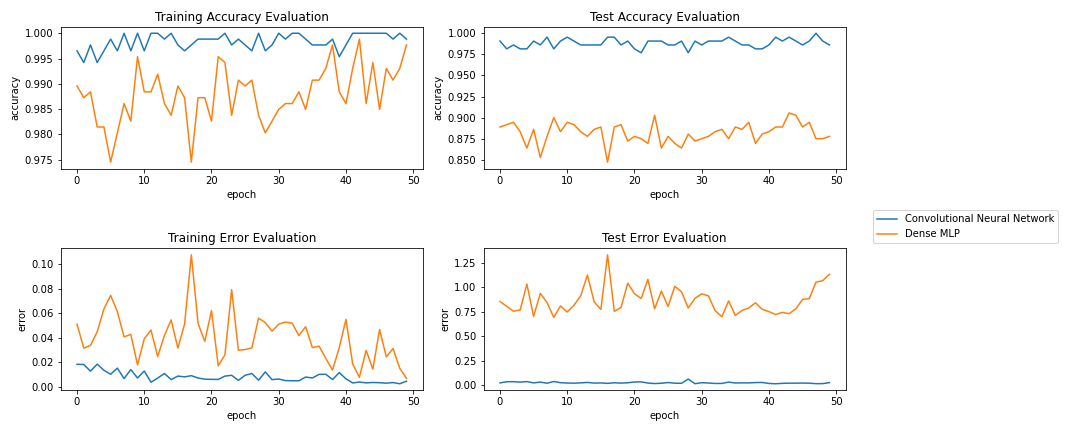
\includegraphics[width= 1.00 \textwidth]{accuracyMeasures.png}
\subsection{CNN Results}
With $\mu=0.0001, \bar{t}=3.23s$
\begin{itemize}
\item \textbf{Average Accuracy (preserved samples}: 92.31\%
\item \textbf{Average Accuracy (randomised samples}: 94.56\%
\end{itemize}

\subsection{Dense Network Results}
With $\mu=0.0001, \textit{dropout}=0.1, \bar{t}=13.15s$
\begin{itemize}
\item \textbf{Average Accuracy (preserved samples}: 81.72\%
\item \textbf{Average Accuracy (randomised samples}: 86.657\%
\end{itemize}

\subsection{LSTM Network Results}
With $\mu=0.0001, \bar{t}=48.26s$
\begin{itemize}
\item \textbf{Average Accuracy (preserved samples}: 70.43\%
\item \textbf{Average Accuracy (randomised samples}: 92.31\%
\end{itemize}


%\section{Limitations}
%\begin{itemize}
%\item Training can currently include different features from the same person's voice as the test set.
%\item The amount of training data currently available is rather limited. Perturbating the existing data could potentially increase accuracy.
%\item Hyper-parameter optimisation will be necessary.
%\item An LSTM solution was implemented but does not run in \texttt{Python 3.8} and I am still troubleshooting compatibility.
%\end{itemize}













\end{document}